%\documentclass[12pt, oneside]{article}   	% use "amsart" instead of "article" for AMSLaTeX format
%\usepackage{geometry}                		% See geometry.pdf to learn the layout options. There are lots.
%\geometry{letterpaper}                   		% ... or a4paper or a5paper or ... 
%\geometry{landscape}                		% Activate for rotated page geometry
%\usepackage[parfill]{parskip}    		% Activate to begin paragraphs with an empty line rather than an indent
%\usepackage{graphicx}				% Use pdf, png, jpg, or eps§ with pdflatex; use eps in DVI mode

\documentclass[%
 reprint,
%superscriptaddress,
%groupedaddress,
%unsortedaddress,
%runinaddress,
%frontmatterverbose, 
%preprint,
%showpacs,preprintnumbers,
%nofootinbib,
%nobibnotes,
%bibnotes,
 amsmath,amssymb,
 aps,
%pra,
%prb,
%rmp,
%prstab,
%prstper,
%floatfix,
]{revtex4-1}

\usepackage{graphicx}% Include figure files
\graphicspath{{Images/}}
\usepackage{float}
\usepackage{dcolumn}% Align table columns on decimal point
\usepackage{bm}% bold math
%\usepackage{hyperref}% add hypertext capabilities
%\usepackage[mathlines]{lineno}% Enable numbering of text and display math
%\linenumbers\relax % Commence numbering lines

%\usepackage[showframe,%Uncomment any one of the following lines to test 
%%scale=0.7, marginratio={1:1, 2:3}, ignoreall,% default settings
%%text={7in,10in},centering,
%%margin=1.5in,
%%total={6.5in,8.75in}, top=1.2in, left=0.9in, includefoot,
%%height=10in,a5paper,hmargin={3cm,0.8in},
%]{geometry}

\usepackage{mathrsfs}
\usepackage{amsmath}

\begin{document}
\bibliographystyle{unsrtnat}

\preprint{APS/123-QED}

\title{Solving the Time-Independent Schrodinger Equation Computationally}

\author{Anne Stratman and Ben Riordan}
\affiliation{%
Computational Lab in Quantum Mechanics, Spring 2018, University of Notre Dame}%

\maketitle								% TeX will automatically convert eps --> pdf in pdflatex		
%\usepackage{amssymb}

%SetFonts

%SetFonts


%\title{Brief Article}
%\author{The Author}
%\date{}							% Activate to display a given date or no date
%\maketitle
%\section{}
%\subsection{}

\noindent \textbf{Introduction: Discrete Basis}\\

\noindent The time-independent Schrodinger equation, given by
\begin{equation}
-\frac{\hbar^2}{2m}\frac{d^2}{dx^2}\psi(x)+V(x)\psi(x)=E\psi(x)
\end{equation}

\noindent can be solved as a matrix diagonalization problem.  This problem can be solved in a discrete basis, or a harmonic oscillator basis.  The solution in the discrete basis is found using inner products of distinct points ($\langle x_i|H|x_j\rangle$).  To solve the problem in the discrete basis, one rewrites the second derivative in the Schrodinger equation in terms of the value of $\psi$ at three discrete points.  The resulting equation can then be used to define diagonal and nondiagonal matrix elements.  Each of these matrix elements is evaluated at a discrete points, and the resulting matrix, is diagonalized.  This gives the Hamiltonian for the potential, or a set of eigenvalues and eigenvectors which correspond to the allowed energies and their wavefunctions.  To begin this process, the second derivative can be rewritten as
\begin{equation}
f''=\frac{f(x+h)-2f(x)+f(x-h)}{h^2}+O(h^2)
\end{equation}
\noindent where \textit{h} is the step size.  Next, we can define minimum and maximum values for the variable \textit{x}, \textit{R}$_{min}$ and \textit{R}$_{max}$, respectively.  For a given number of steps \textit{N}, the step size \textit{h} can be defined by
\begin{equation}
h=\frac{R_{max}-R_{min}}{N}
\end{equation}

\noindent Defining an arbitrary value of \textit{x} as \textit{x}=\textit{R}$_{min}$+\textit{kh}, \textit{k}=1,2,...,\textit{N}$_{step}$-1, the Schrodinger equation can be rewritten for \textit{x}$_k$ as
\begin{multline}
-\frac{\hbar^2}{2m}\frac{\psi(x_k+h)-2\psi(x_k)+\psi(x_k-h)}{h^2}+V(x)\psi(x_k)\\
=E\psi(x_k)
\end{multline}
\noindent or, more compactly,
\begin{equation}
-\frac{\hbar^2}{2m}\frac{\psi_{k+1}-2\psi_k+\psi_{k-1}}{h^2}+V_k\psi_k=E\psi_k
\end{equation}
\noindent where \textit{$\psi$}$_k$=\textit{$\psi$}(\textit{x}$_k$) and \textit{$\psi$}$_{k\pm1}$=\textit{$\psi$}(\textit{x}$_k$$\pm$\textit{h}).  Next, we can define diagonal matrix elements:
\begin{equation}
d_k=\frac{\hbar^2}{2m}\frac{2}{h^2}+V_k
\end{equation}
\noindent and non-diagonal matrix elements:
\begin{equation}
e_k=-\frac{\hbar^2}{2m}\frac{1}{h^2}
\end{equation}

\noindent This gives the following form for the Schrodinger equation:
\begin{equation}
d_k\psi_k+e_{k-1}\psi_{k-1}+e_{k+1}\psi_{k+1}=E\psi_k
\end{equation}
\noindent and allows us to solve the Schrodinger equation as a matrix eigenvalue problem.\\

\begin{figure}
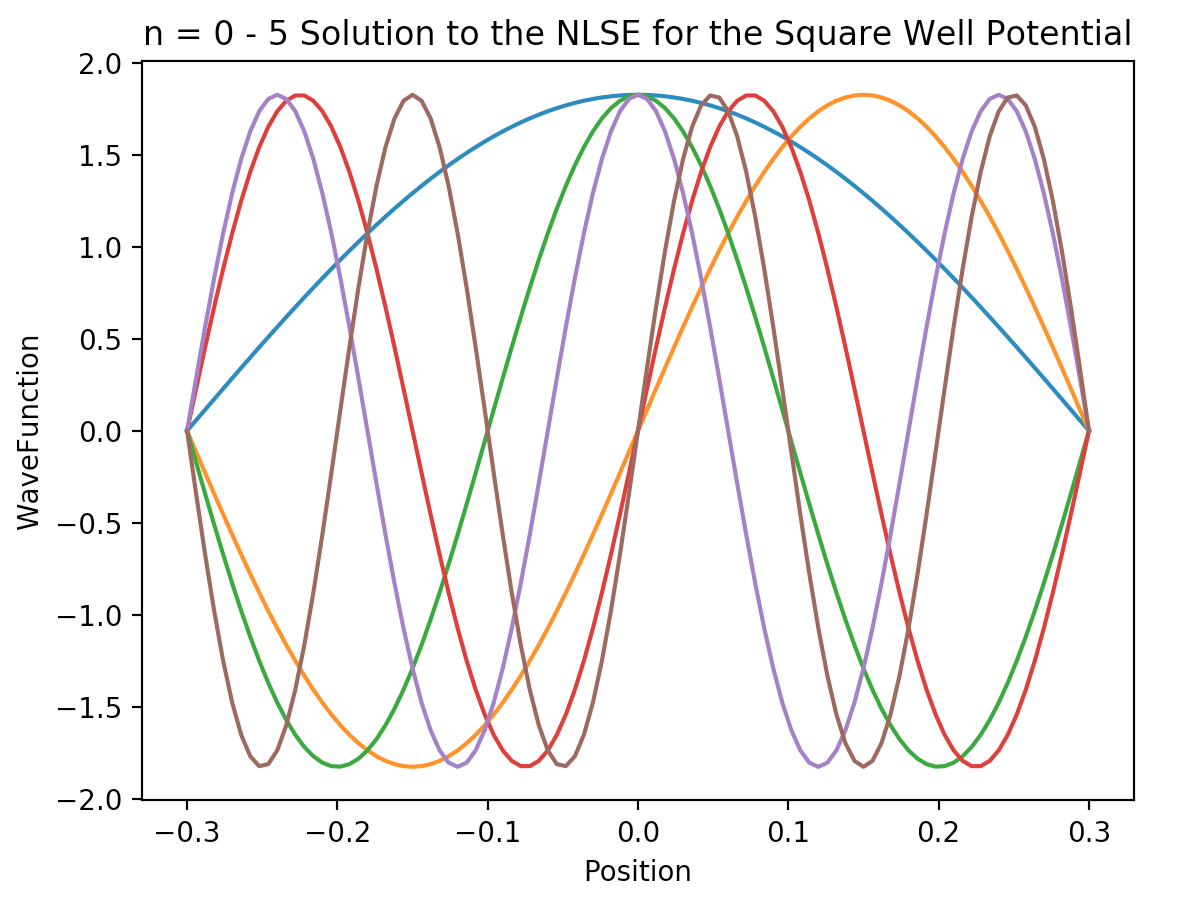
\includegraphics[width=9cm]{DiscreteBasisSquareWell}
\caption{Square well solved in the discrete basis, using 100 points}
\end{figure}
\begin{figure}
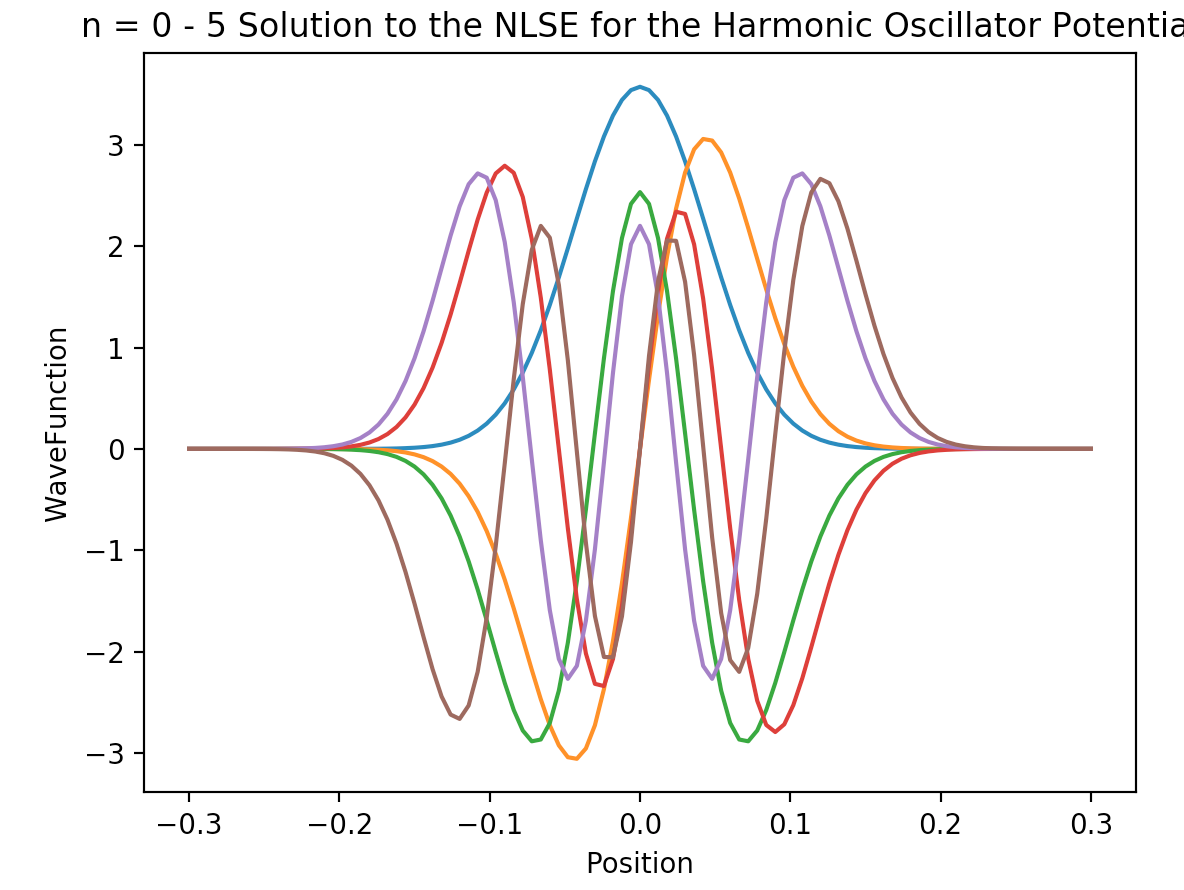
\includegraphics[width=9cm]{DiscreteBasisHarmonicOscillator}
\caption{Harmonic oscillator solved in the discrete basis, using 100 points}
\end{figure}

\noindent \textbf{Introduction: Harmonic Oscillator Basis}\\

\noindent The harmonic oscillator basis solution to the Schrodinger equation uses inner products of wavefunctions ($\langle\psi_m|H|\psi_n\rangle$) to find the matrix elements, and transforms the resulting Hamiltonian into the harmonic oscillator basis.  The solutions to the harmonic oscillator are given by the equation
\begin{equation}
\psi_n(x)=\Bigg{(}\frac{m\omega}{\pi\hbar}\Bigg{)}^{1/4}\frac{1}{\sqrt{2^n n!}}H_n(\xi)e^{-\xi^2/2}
\end{equation}
\noindent where
\begin{equation}
\xi=\sqrt{\frac{m\omega}{\hbar}}x
\end{equation}
The matrix elements are found by taking the inner product $\langle$\textit{m}$|$\textit{H}$|$\textit{n}$\rangle$, which yields
\begin{multline}
\frac{1}{2m}\langle n|p^2|m \rangle + \langle n|V|m \rangle \\
=-\frac{\hbar\omega}{4}[\sqrt{m+1}\sqrt{m+2}\delta_{n,m+2}-\sqrt{m+1}\sqrt{m+1}\delta_{m,n}\\
-\sqrt{m}\sqrt{m}\delta{m,n}+\sqrt{m}\sqrt{m+1}\delta_{n,m-2}] \\
+ \int_{-\infty}^{\infty}\psi_n^*(x)V(x)\psi_m(x)dx
\end{multline}
After the matrix elements are found, the resulting matrix is diagonalized to give the Hamiltonian, which has dimensions (number of wavefunctions, number of wavefunctions).  This matrix is then multiplied by a transformation matrix with dimensions (number of steps, number of wavefunctions) to give the solution in the harmonic oscillator basis.\\

\begin{figure}
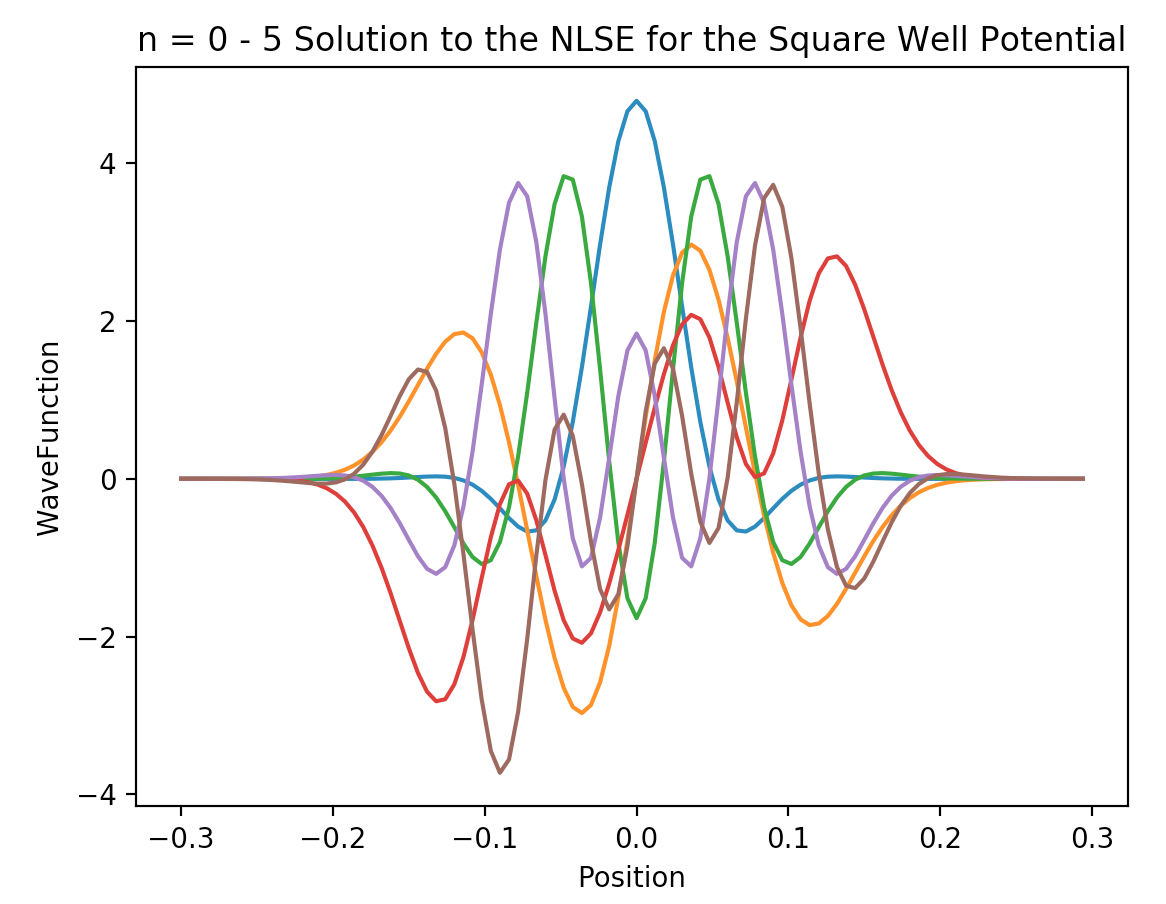
\includegraphics[width=9cm]{HOBasisSquareWell}
\caption{Square well solved in the harmonic oscillator basis, using 5 basis functions}
\end{figure}
\begin{figure}
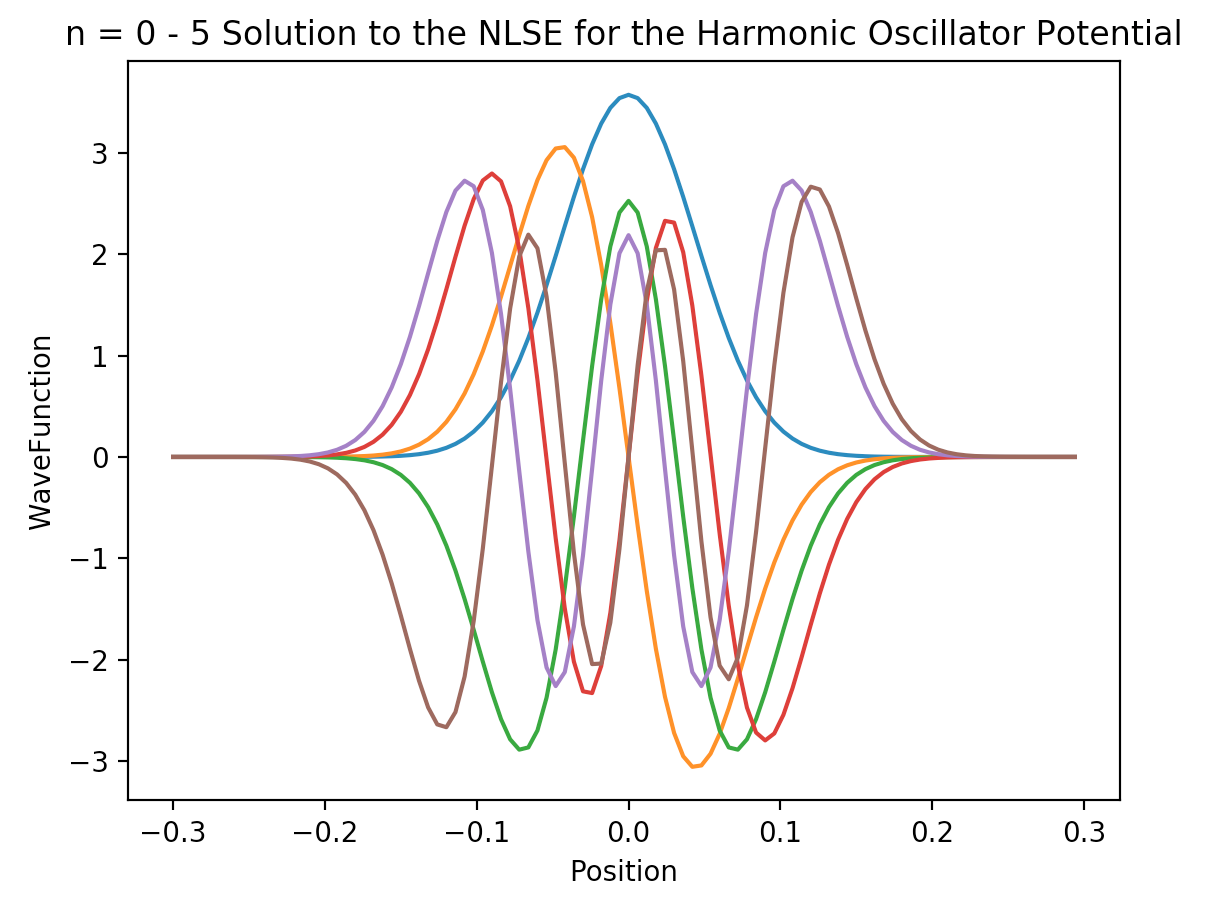
\includegraphics[width=9cm]{HOBasisHarmonicOscillator}
\caption{Harmonic oscillator solved in the harmonic oscillator basis, using 5 basis functions}
\end{figure}

\noindent \textbf{Programming}\\

\noindent We structured our code by defining two classes, one for the discrete basis and one for the harmonic oscillator basis.  Both classes have attributes \textit{potential} (the potential function), \textit{x}$_{min}$, \textit{x}$_{max}$, \textit{n steps} (number of steps - used for determining matrix dimensions), \textit{particle mass}, \textit{h} (to determine the step size), and \textit{xPoints} (to determine the points to evaluate the wavefunction at).  The harmonic oscillator class also has attributes \textit{omega} and \textit{hbar}.\\

\noindent The discrete class includes separate functions for finding each element of the matrix, creating the matrix, and diagonalizing the matrix.  The ``matrix element finder" function uses equations (6) and (7) to find the diagonal and off-diagonal matrix elements, respectively.  The ``matrix maker" function creates a zero matrix of dimensions (\textit{n steps} + 1, \textit{n steps} + 1).  This function then calls ``matrix element finder" to fill in the diagonal and off-diagonal elements of the matrix, giving the Hamiltonian.  The ``matrix solver" function uses Numpy's ``linalg.eigh" function to diagonalize the Hamiltonian, and then takes the transpose of this matrix, giving the eigenvectors and eigenvalues.\\

\noindent The harmonic oscillator class first includes a function for defining the harmonic oscillator wavefunction.  This function calls a separate module to evaluate Hermite polynomials.  The momentum and potential inner products corresponding to the Hamiltonian are defined in separate functions.  In addition, a function for defining (NOT integrating) the integrand in the potential term is defined separately.  A ``matrix element finder" function adds the momentum operator and potential operator terms, and ``matrix maker" and ``matrix solver" functions are defined similarly to those in the discrete class.  The zero matrix initially created by ``matrix maker" has dimensions (number of functions, number of functions).\\

\noindent The plotting function, defined outside the two classes, includes a component for transforming the Hamiltonian given by the harmonic oscillator solver into the harmonic oscillator basis.  The transformation component takes the Numpy dot product of a transformation matrix and the eigenvector matrix of given by the harmonic oscillator solver.  The transformation matrix has dimensions (number of steps, number of functions), with elements representing each of the harmonic oscillator functions evaluated at a different point; thus multiplying the transformation matrix and the eigenvector matrix gives the solution in the harmonic oscillator basis.\\

\noindent \textbf{Analysis of Correctness}\\

\noindent To test whether this program gives the correct results, we used our code to solve problems with known solutions, specifically the infinite square well and the harmonic oscillator.  Various plots of our solutions are shown throughout the report.  \textit{Figure 5} and \textit{Figure 6}, which show the correct solutions to the infinite square well and the harmonic oscillator, respectively, are taken from Griffiths' \textit{Introduction to Quantum Mechanics}.\\

\noindent As shown in \textit{Figure 3}, the solution to the square well potential solved in the harmonic oscillator basis is not correct, which is expected.  When solving the TISE in the harmonic oscillator basis, one should integrate the inner product out to positive and negative infinity (the SciPy ``integrate.quad" function does this).  When solving the square well, however, one should just integrate the inner products between the endpoints of the well.  Therefore, the limits of integration in the harmonic oscillator basis are much too large for solving square well potentials, and should not yield the correct results.\\

\noindent \textit{Figure 2} and \textit{Figure 4} show that certain solutions for the harmonic oscillator potential in the harmonic oscillator basis are negative solutions of the results from the discrete basis.  Since any ``negative" solution to an eigenvalue problem is still a solution, though, this is no cause for concern.  \textit{Figure 5} shows the eigenvalues of the square well as a function of \textit{n} (corresponding to the \textit{n}$^{th}$ wavefunction).  \textit{Figure 6} shows the eigenvalues of the harmonic oscillator as a function of \textit{n}.  As expected, these are a line, since for the harmonic oscillator \textit{E}$_n$ = (\textit{n} + $\frac{1}{2}$)$\hbar\omega$.\\

\begin{figure}
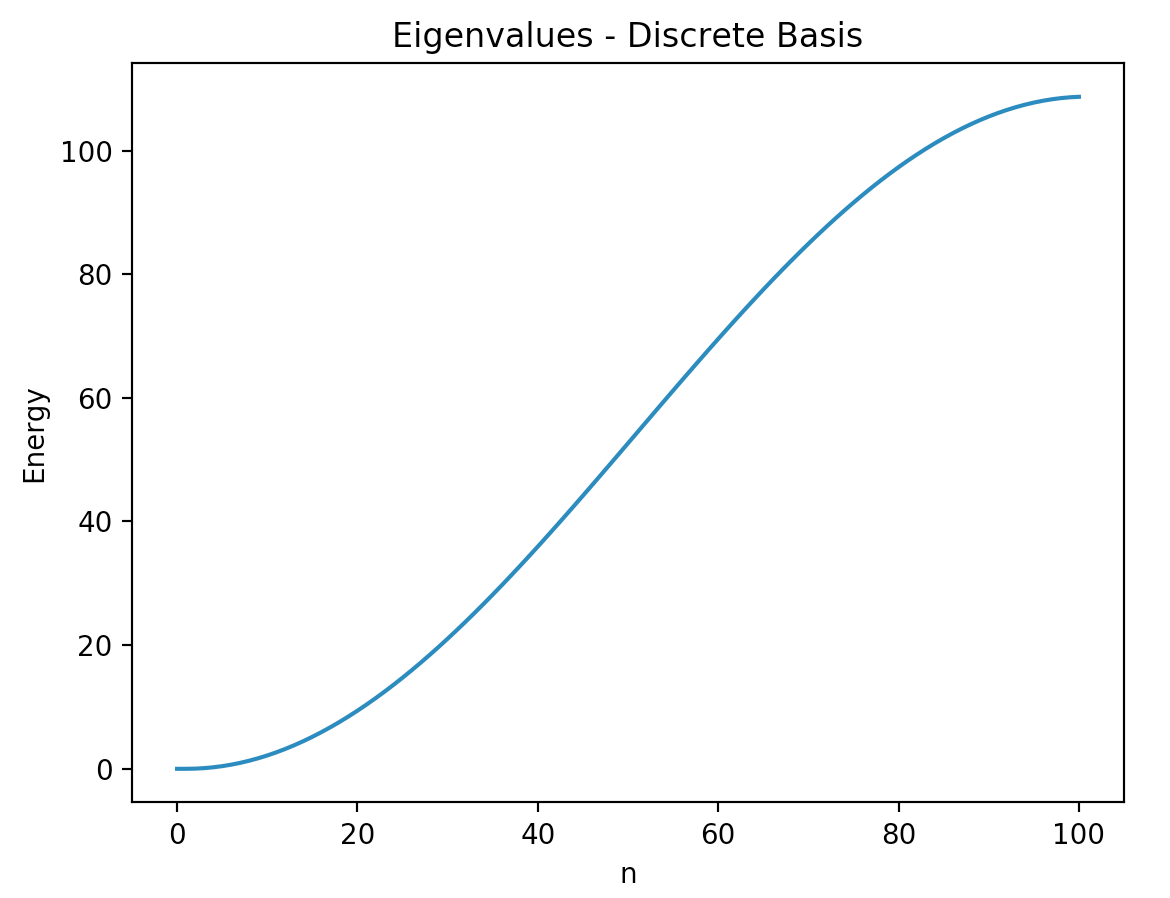
\includegraphics[width=9cm]{DiscreteSquareWellEigenvalues}
\caption{Eigenvalues of the square well potential, solved in the discrete basis using 100 points}
\end{figure}
\begin{figure}
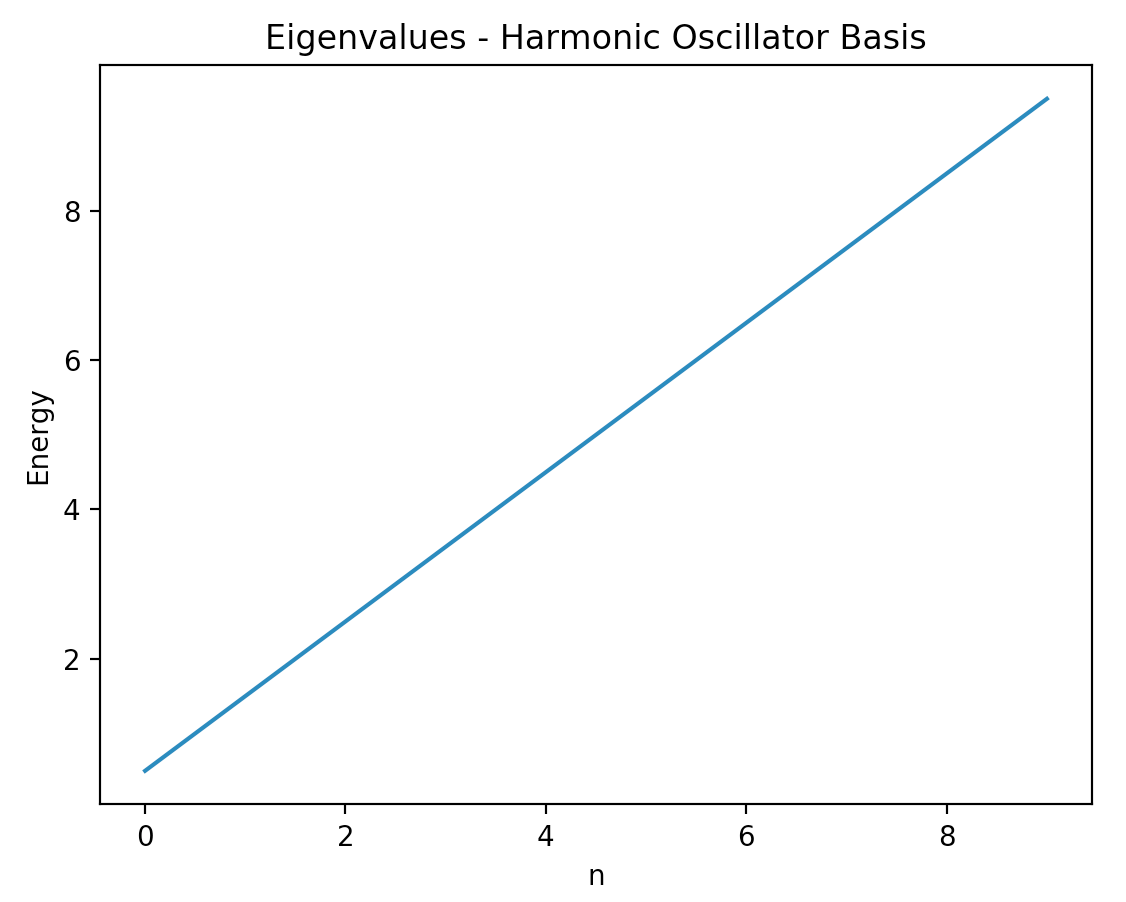
\includegraphics[width=9cm]{HOHarmonicOscillatorEigenvalues}
\caption{Eigenvalues of the harmonic oscillator potential, solved in the harmonic oscillator basis using 5 basis functions}
\end{figure}

\noindent To achieve reasonable numerical precision, at least 100 points should be used when solving a potential in the discrete basis.  This yields at least 100 points at which the code can evaluate the wavefunction solutions and plot the results.  \textit{Figure 5} and \textit{Figure 6} show the convergence of the eigenvalues for different numbers of points for the square well and harmonic oscillator potentials, respectively, solved in the discrete basis.  In the harmonic oscillator basis, SciPy's ``integrate.quad" function integrates the inner products of wavefunctions and the potential out to positive and negative infinity, which effectively takes the place of evaluating the inner products at many discrete points, as is done in the discrete basis solver.  Solutions to potentials in the harmonic oscillator basis vary depending on the number of basis functions used, and because the inner products are already integrated out to extremely large values, a much smaller number of basis functions yields an accurate solution.  We found accurate solutions using as few as five basis functions.\\

\begin{figure}
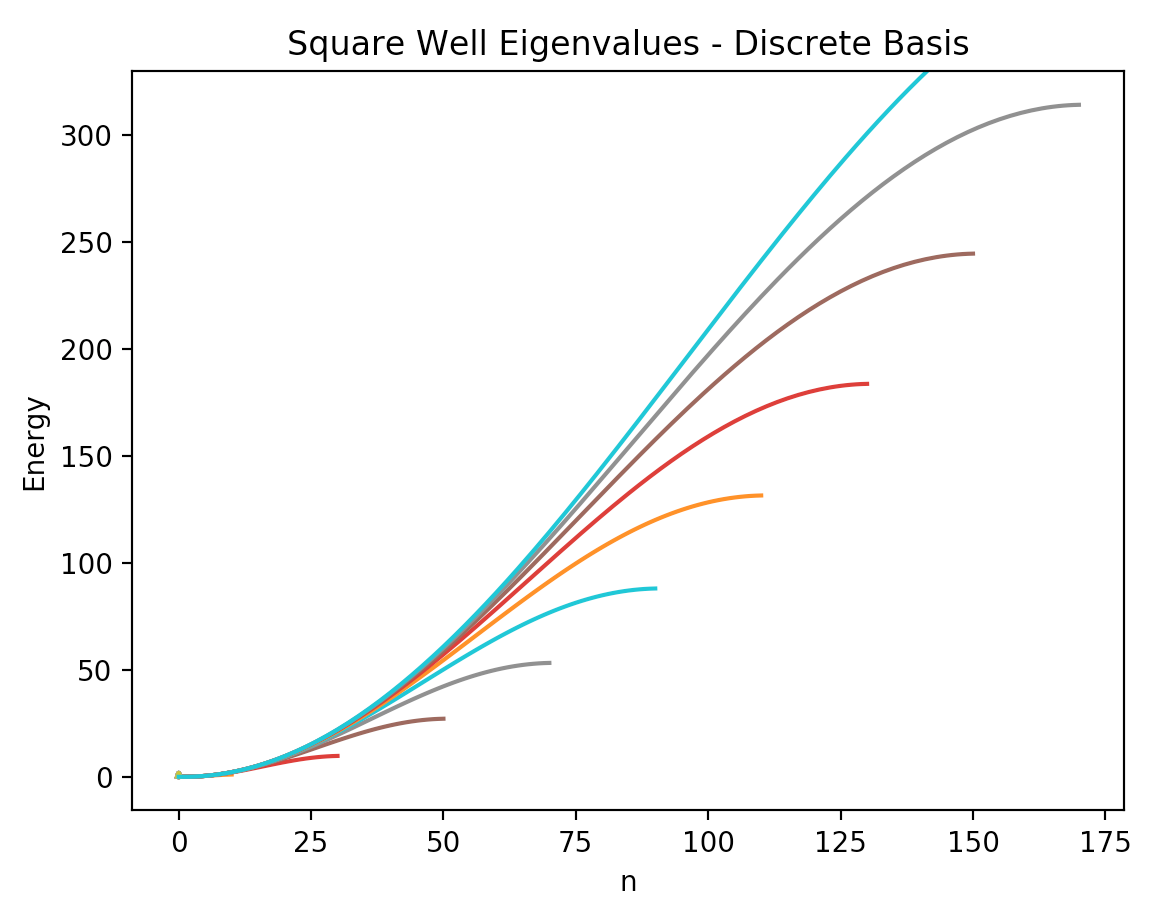
\includegraphics[width=9cm]{DiscreteSquareWellEigenvaluesConvergence}
\caption{Convergence of eigenvalues for the square well potential solved in the discrete basis.  Minimum number of steps = 10, maximum number of steps = 190, plotted in increments of 20.}
\end{figure}
\begin{figure}
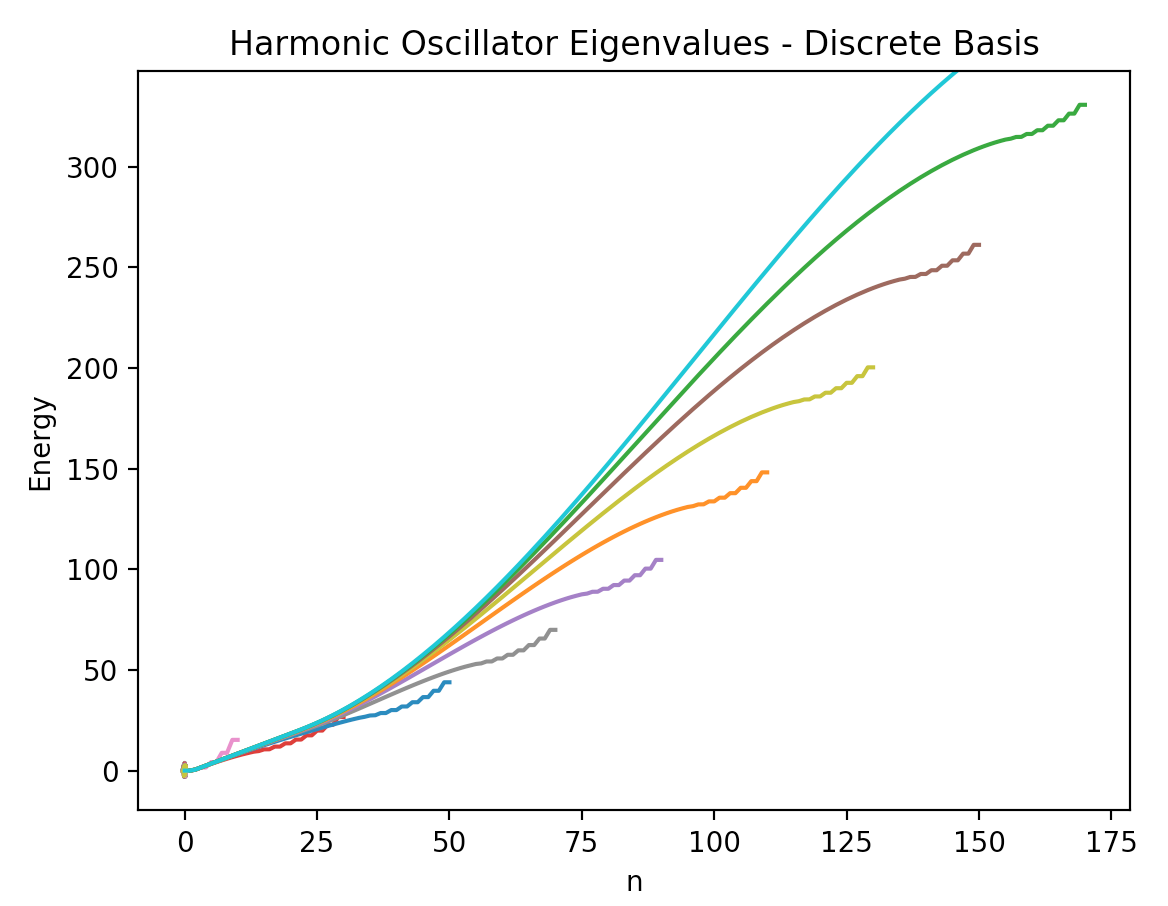
\includegraphics[width=9cm]{DiscreteHarmonicOscillatorEigenvaluesConvergence}
\caption{Convergence of eigenvalues for the harmonic potential solved in the discrete basis.  Minimum number of steps = 10, maximum number of steps = 190, plotted in increments of 20.}
\end{figure}


%\begin{figure}
%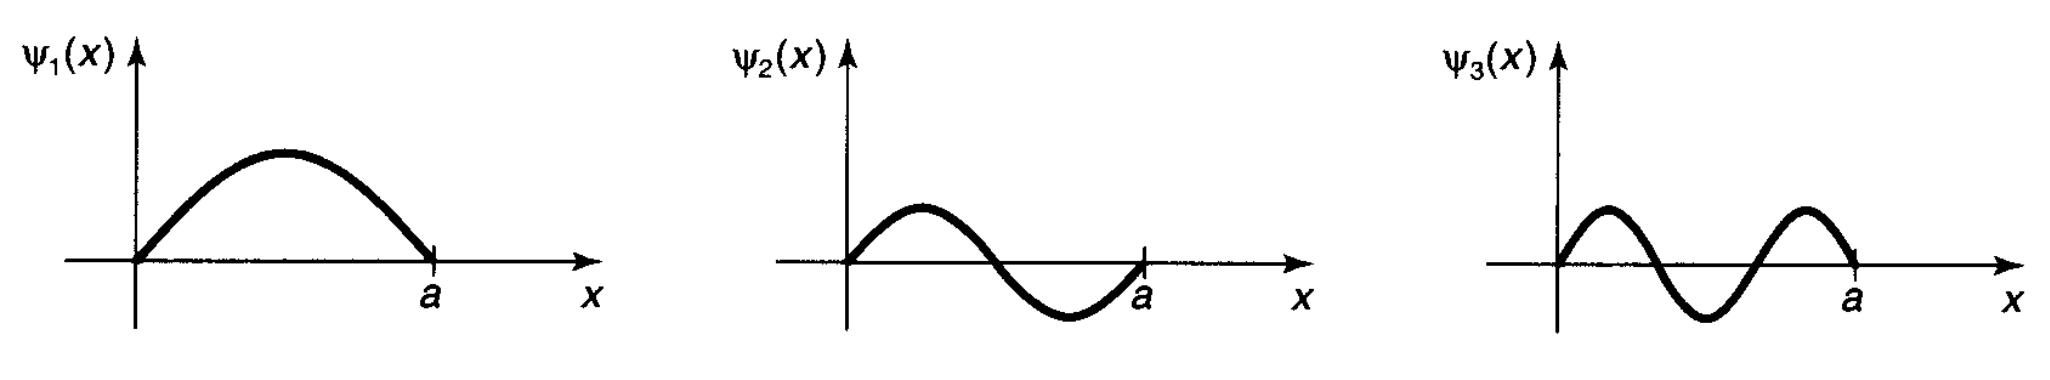
\includegraphics[width=9cm]{KnownSquareWellSolutions}
%\caption{Known solutions to the infinite square well}
%\end{figure}
%\begin{figure}
%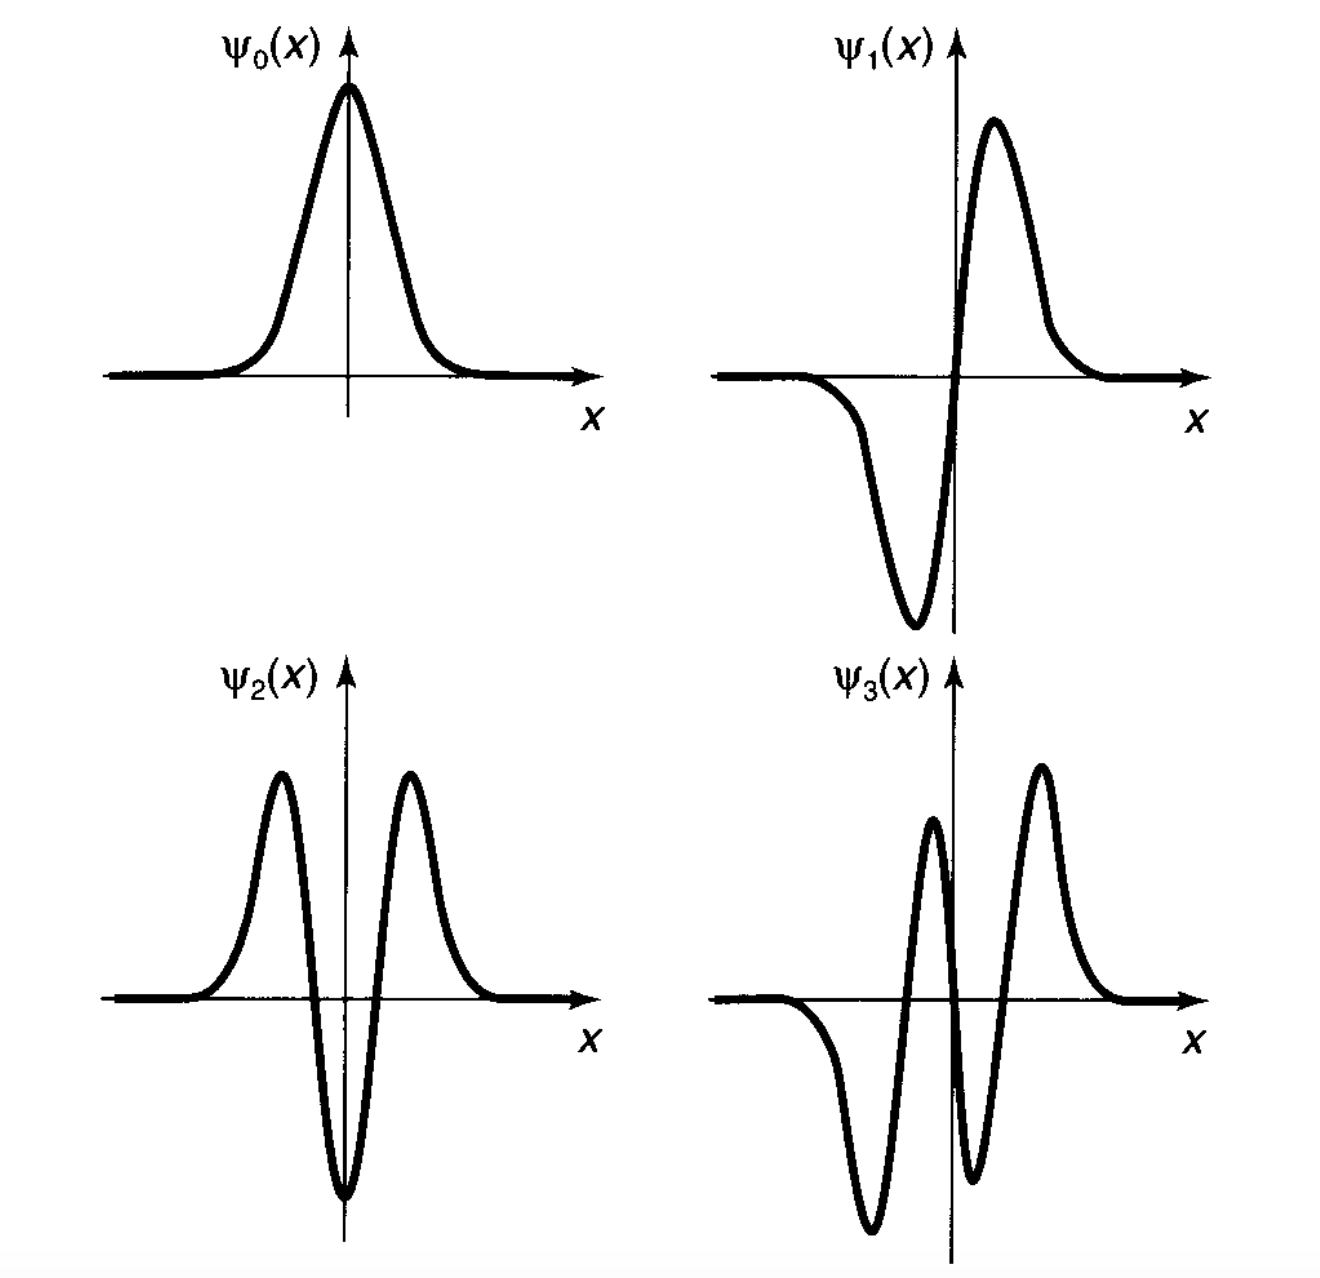
\includegraphics[width=9cm]{KnownHarmonicOscillatorSolutions}
%\caption{Known solutions to the harmonic oscillator potential}
%\end{figure}
\begin{figure}
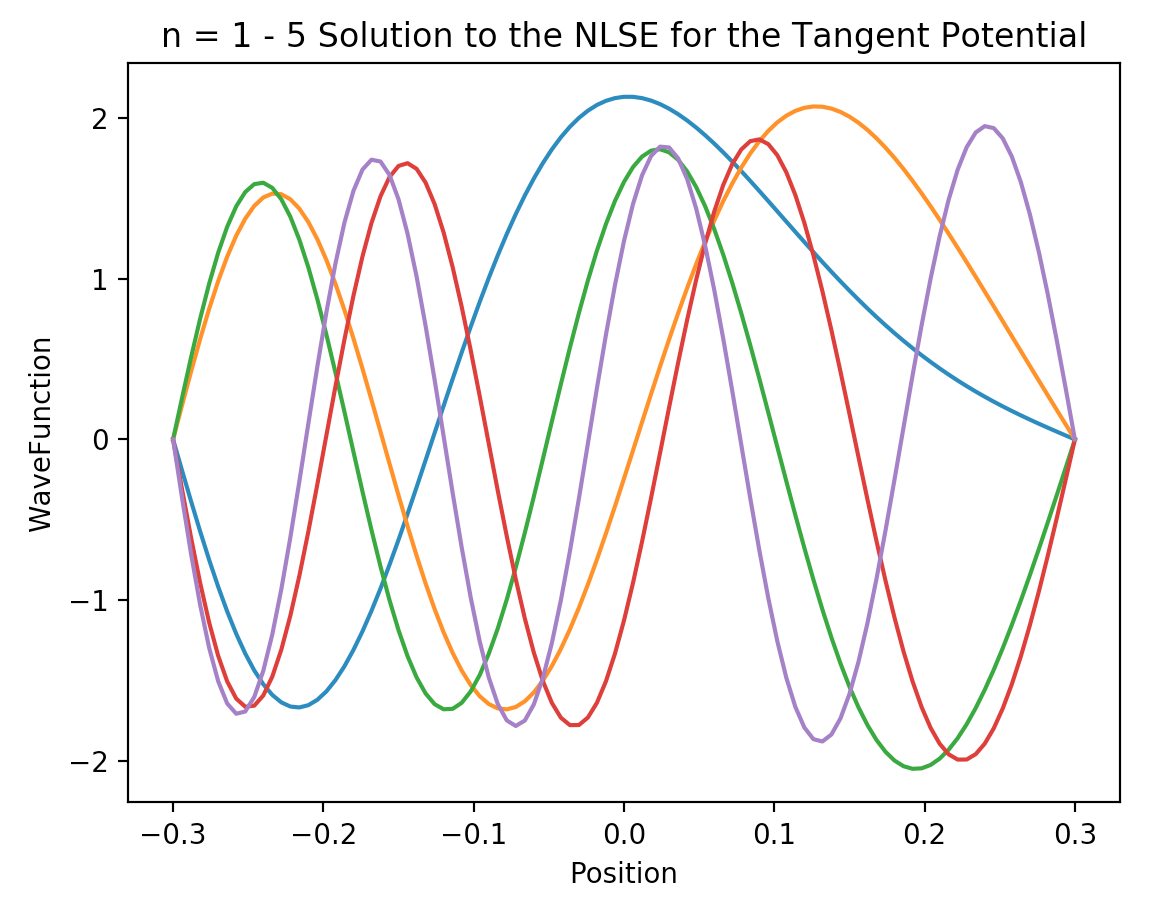
\includegraphics[width=9cm]{DiscreteBasisTangent}
\caption{Tangent potential solved in the discrete basis, using 100 points}
\end{figure}
\begin{figure}
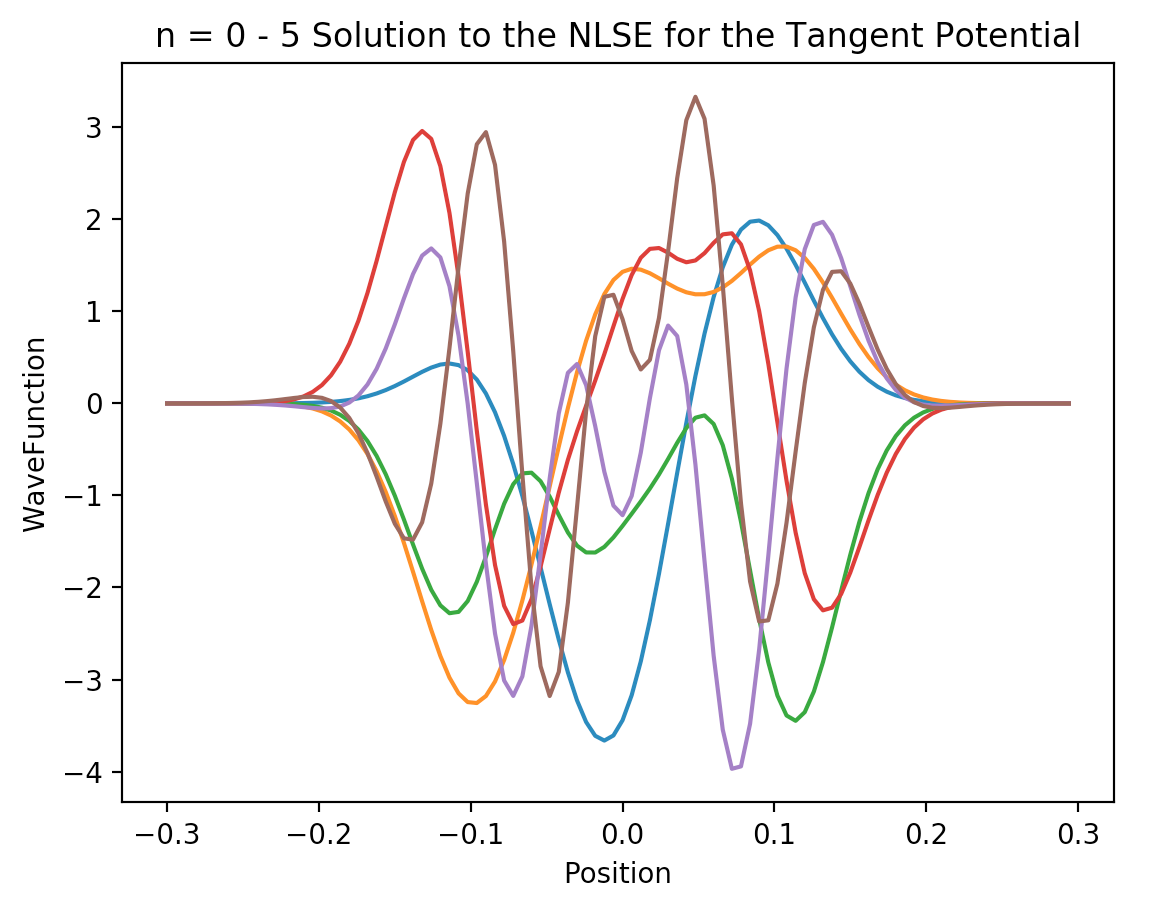
\includegraphics[width=9cm]{HOBasisTangent}
\caption{Tangent potential solved in the harmonic oscillator basis, using 5 basis functions}
\end{figure}

\noindent We also used this code to solve the tangent potential $V(x) = tan(x)$ in both the discrete and harmonic oscillator bases (\textit{Figure 9} and \textit{Figure 10}).\\

\noindent \textbf{Units}\\

\noindent The units of mass in this code are keV.  In the harmonic oscillator basis, we worked in units such that $\hbar$ and $\omega$ were equal to 1.\\

\noindent \textbf{Conclusion}\\

\noindent The Schrodinger equation can be solved computationally through matrix diagonalization in multiple bases.  We have developed a program to solve the time-independent Schrodinger equation in two bases - the discrete basis and the harmonic oscillator basis.  As shown in our plots, the solutions given by our code are consistent with known solutions.  Therefore, this code can be used to solve the Schrodinger equation for potentials that can only be solved numerically.\\

\noindent \textbf{Acknowledgements}\\

\noindent I would like to thank my partner, Ben, for working with me for eight entire weeks on this project, and for spending hours trying to figure out why our solutions were ``wrong" (i.e. negative) when they were actually correct because we both forgot how linear algebra worked.  I would also like to thank Sam and Judah, for helping us fix our harmonic oscillator basis when their code worked and ours didn't.  Finally, I would like to thank Patrick for his guidance in this project (\#eigenboisneedhelp), and for bringing us doughnuts.  (Please bring more doughnuts.)  Eigenbois out.

\end{document}